\documentclass[11pt]{article}

\usepackage[a4paper,margin=1in]{geometry}
\usepackage{amsmath}
\usepackage{graphicx}
\usepackage{amssymb}
\usepackage{parskip}
\usepackage[table]{xcolor}
\usepackage{tikz}
\usetikzlibrary{arrows.meta, positioning, shapes.geometric, calc, fit}
\usepackage[most]{tcolorbox}
\usepackage{titlesec}
\usepackage{enumitem}
\usepackage{booktabs}
\usepackage{array}
\usepackage{hyperref}

% ---------- Colors ----------
\definecolor{deepblue}{HTML}{1B3B6F}
\definecolor{accent}{HTML}{2E86AB}
\definecolor{accent2}{HTML}{E07A3F}
\definecolor{soft}{HTML}{F4F7FB}
\definecolor{soft2}{HTML}{FFF4EC}
\definecolor{linegray}{HTML}{D6DEE8}
\definecolor{textgray}{HTML}{333333}
\definecolor{codebg}{HTML}{1B3B6F}
\definecolor{codefg}{HTML}{F4F7FB}

% ---------- Section styling ----------
\titleformat{\section}
  {\Large\bfseries\color{deepblue}}
  {}{0em}{}[{\color{accent}\titlerule[1.2pt]}]
\titlespacing*{\section}{0pt}{18pt}{10pt}

\titleformat{\subsection}
  {\large\bfseries\color{accent}}
  {\thesubsection}{0.6em}{}
\titlespacing*{\subsection}{0pt}{14pt}{6pt}

% ---------- Reusable boxes ----------
\newtcolorbox{codebox}{
  colback=codebg, colframe=codebg,
  coltext=codefg,
  fonttitle=\bfseries,
  boxrule=0pt, arc=3pt, outer arc=3pt,
  left=8pt, right=8pt, top=6pt, bottom=6pt,
  fontupper=\ttfamily\small
}

\newtcolorbox{stepbox}[1]{
  colback=soft, colframe=deepblue,
  boxrule=0.8pt, arc=3pt, outer arc=3pt,
  left=10pt, right=10pt, top=6pt, bottom=6pt,
  title={#1}, fonttitle=\bfseries\color{white},
  colbacktitle=deepblue, coltitle=white
}

\newtcolorbox{plainbox}{
  colback=soft, colframe=accent,
  boxrule=0.8pt, arc=3pt, outer arc=3pt,
  left=10pt, right=10pt, top=6pt, bottom=6pt
}

\newtcolorbox{warnbox}{
  colback=soft2, colframe=accent2,
  boxrule=0.8pt, arc=3pt, outer arc=3pt,
  left=10pt, right=10pt, top=6pt, bottom=6pt
}

\hypersetup{
  colorlinks=true, linkcolor=deepblue, urlcolor=deepblue
}

\begin{document}

% ---------- Title ----------
\begin{center}
  {\Huge\bfseries\color{deepblue} Pairwise vs.\ Multi-Preference Optimization}\\[4pt]
  {\color{accent}\rule{0.4\linewidth}{1pt}}
\end{center}
\vspace{8pt}

\section*{Setup: One Prompt, Several Responses}

Suppose we have one prompt:

\begin{center}
\textit{Prompt: Explain why the sky is blue.}
\end{center}

The model generates several candidate answers, each with a reward score:

\begin{center}
\renewcommand{\arraystretch}{1.3}
\begin{tabular}{>{\bfseries\color{deepblue}}c c}
\toprule
\rowcolor{soft} Response & Reward \\
\midrule
A & 9 \\
B & 8 \\
C & 5 \\
D & 2 \\
\bottomrule
\end{tabular}
\end{center}

The question is: \textbf{how do we turn this ranked list into a training signal?} The two approaches below answer this differently.

\section*{Pairwise Preference Optimization}

\subsection*{Basic Idea}

In pairwise preference optimization, training uses \textbf{two} responses at a time:

\[
(x, y_w, y_l)
\]

where $y_w$ is the preferred/winner response and $y_l$ is the rejected/loser response. This is the basic setup behind methods such as \textbf{DPO}: for each training example, you have one chosen response and one rejected response.

\subsection*{Example}

\begin{stepbox}{Picking a single pair}
From our four responses, we might pick:
\[
A \succ D.
\]
The training signal is simply:
\begin{center}
\textit{``Make $A$ more likely than $D$.''}
\end{center}
\end{stepbox}

\begin{center}
\resizebox{0.45\textwidth}{!}{%
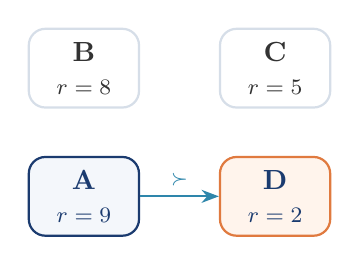
\begin{tikzpicture}[
  node distance=8mm and 10mm,
  box/.style={rectangle, rounded corners=6pt, draw=deepblue, thick,
              fill=soft, minimum width=14mm, minimum height=10mm,
              align=center, font=\bfseries\color{deepblue}},
  loser/.style={box, fill=soft2, draw=accent2},
  arrow/.style={-{Stealth[length=2.2mm]}, thick, color=accent}
]
  \node[box] (a) {A \\ \footnotesize $r=9$};
  \node[loser, right=of a] (d) {D \\ \footnotesize $r=2$};
  \node[box, draw=linegray, fill=white, font=\bfseries\color{textgray}, above=6mm of a] (b) {B \\ \footnotesize $r=8$};
  \node[box, draw=linegray, fill=white, font=\bfseries\color{textgray}, above=6mm of d] (c) {C \\ \footnotesize $r=5$};

  \draw[arrow] (a) -- node[above, font=\scriptsize\itshape\color{textgray}] {$\succ$} (d);
\end{tikzpicture}%
}
\end{center}

\subsection*{The Limitation}

\begin{warnbox}
We started with four responses, $A, B, C, D$, but the optimization step only directly compared \textbf{$A$ vs.\ $D$}. Information about $B$ and $C$ — both of which carry useful signal about response quality — can be lost.
\end{warnbox}

\section*{Multi-Preference Optimization}

\subsection*{Basic Idea}

Multi-preference optimization asks a natural question:

\begin{center}
\textit{``Why compare only one winner and one loser when we have many responses with different quality?''}
\end{center}

Instead of a single pair, we consider a \textbf{group} of responses on each side.

\subsection*{Example}

\begin{stepbox}{Forming preference sets}
From the same four responses, we can form:
\[
Y^+ = \{A, B\} \qquad \text{and} \qquad Y^- = \{C, D\}.
\]
Optimization now learns something closer to
\[
\{A, B\} \ \text{preferred over} \ \{C, D\},
\]
rather than only $A \succ D$.
\end{stepbox}

\begin{center}
\resizebox{0.85\textwidth}{!}{%
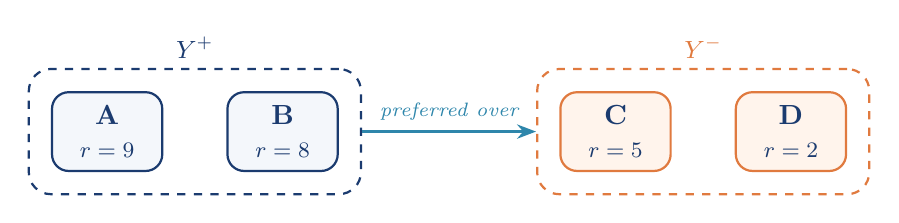
\begin{tikzpicture}[
  node distance=6mm and 10mm,
  box/.style={rectangle, rounded corners=6pt, draw=deepblue, thick,
              fill=soft, minimum width=14mm, minimum height=10mm,
              align=center, font=\bfseries\color{deepblue}},
  loser/.style={box, fill=soft2, draw=accent2},
  groupbox/.style={rectangle, rounded corners=8pt, draw=deepblue, thick, dashed,
                    inner sep=8pt},
  grouplbox/.style={groupbox, draw=accent2},
  arrow/.style={-{Stealth[length=2.4mm]}, very thick, color=accent}
]
  \node[box] (a) {A \\ \footnotesize $r=9$};
  \node[box, right=8mm of a] (b) {B \\ \footnotesize $r=8$};
  \node[loser, right=28mm of b] (c) {C \\ \footnotesize $r=5$};
  \node[loser, right=8mm of c] (d) {D \\ \footnotesize $r=2$};

  \node[groupbox, fit={(a) (b)}, label={[font=\small\bfseries\color{deepblue}]above:$Y^+$}] (gplus) {};
  \node[grouplbox, fit={(c) (d)}, label={[font=\small\bfseries\color{accent2}]above:$Y^-$}] (gminus) {};

  \draw[arrow] (gplus) -- node[above, font=\scriptsize\itshape\color{textgray}] {preferred over} (gminus);
\end{tikzpicture}%
}
\end{center}

\end{document}